\documentclass[12pt]{article}

%Standard Stefanos Packages
\usepackage[utf8]{inputenc}
\usepackage{dirtytalk}
\usepackage{amsmath}
\usepackage{mathtools}  
\mathtoolsset{showonlyrefs} 
\usepackage{graphicx}
\usepackage{mdframed}
\usepackage{lipsum}
\usepackage{cancel}
\usepackage{systeme}
\usepackage{pgfplots}
\usepackage{textcomp}
\usepackage{geometry}
\usetikzlibrary{arrows}
\geometry{a4paper}
\graphicspath{ {./res/} }
\usepackage{float}
\restylefloat{table}
\newcommand{\comment}[1]{%
	\text{\phantom{(#1)}} \tag{#1}
}
\usepackage{subcaption}
\usepackage{graphicx}
\title{\line(1,0){450}\\ CS3DS19 - Data Science Algorithms and Tools \\ \large{Major Coursework }  \\\line(1,0){450} \\2021/2022}
\usepackage{pgfplots}
\author{Student ID: 27020363}
\newmdtheoremenv{note}{Note}
\pgfplotsset{compat=1.17}

%Extra Packages
\usepackage{tikz}
\usetikzlibrary{automata,positioning}

\usepackage{listings}
\usepackage{xcolor}

\definecolor{dkgreen}{rgb}{0,0.6,0}
\definecolor{gray}{rgb}{0.5,0.5,0.5}
\definecolor{mauve}{rgb}{0.58,0,0.82}

\usepackage{mathptmx}
\usepackage{setspace}
\setstretch{1.15}

\lstdefinestyle{myScalastyle}{
	frame=tb,
	language=scala,
	aboveskip=3mm,
	belowskip=3mm,
	showstringspaces=false,
	columns=flexible,
	basicstyle={\small\ttfamily},
	numbers=none,
	numberstyle=\tiny\color{gray},
	keywordstyle=\color{blue},
	commentstyle=\color{dkgreen},
	stringstyle=\color{mauve},
	frame=single,
	breaklines=true,
	breakatwhitespace=true,
	tabsize=3,
}
\begin{document}
	\maketitle
	\pagebreak
	
	\section{Task 1}
		
		In this Section, the  main parts of the workflow will be explained.
		\begin{center}
%			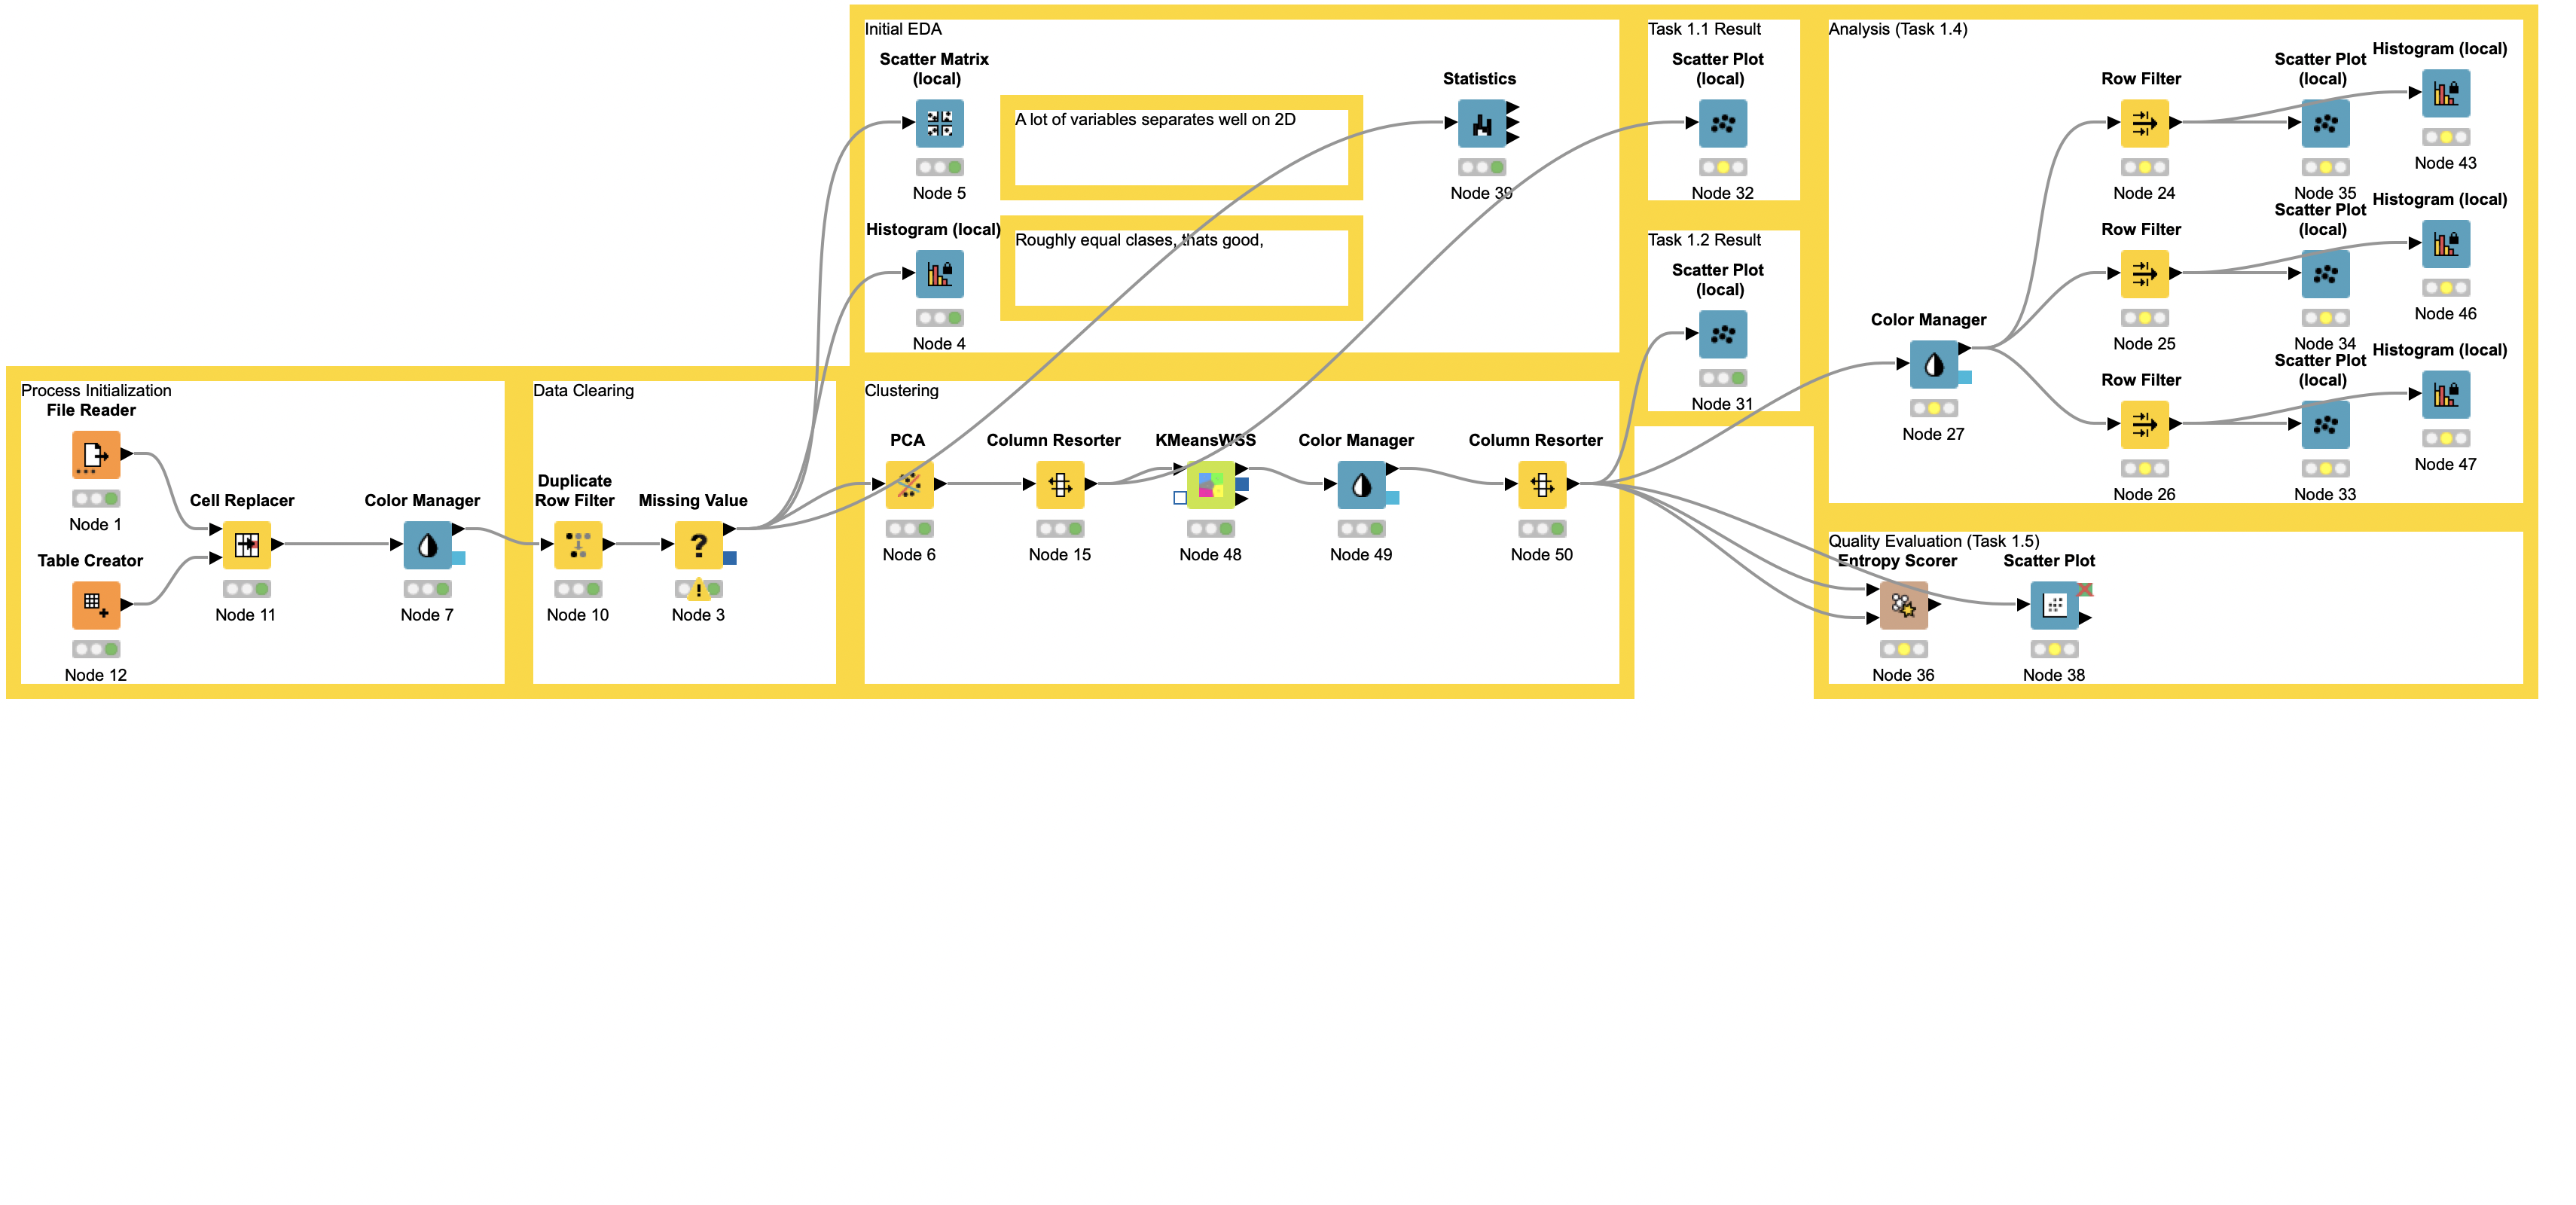
\includegraphics[scale=0.26]{res/workflow}
		\end{center}
		The workflow is splitted into 7 Stages. Those are
		\begin{itemize}
			\item Process Initialization : Read files, and transform the type of the class into string(was number). Finally we assign the initial colours for the subsequent plots, based on the classes field given by the dataset
			\item Data Clearing : Standard data clearing techniques, Drop duplicate data and missing values(by dropping all the rows involving missing data).
			\item Initial EDA : Some useful statistics that i used to get myself familliar with the data and their properties
			\item Clustering : PCA and KMeans Nodes(Futher Explaned below)
			\item Analysis : Evaluation of error, Classes distribution per cluster and histograms
			\item Quality Evaluation : Entropy scorer(Entropy/purity)
		\end{itemize}
	
	\section*{Task 1.1 : plot1}
	
%	 	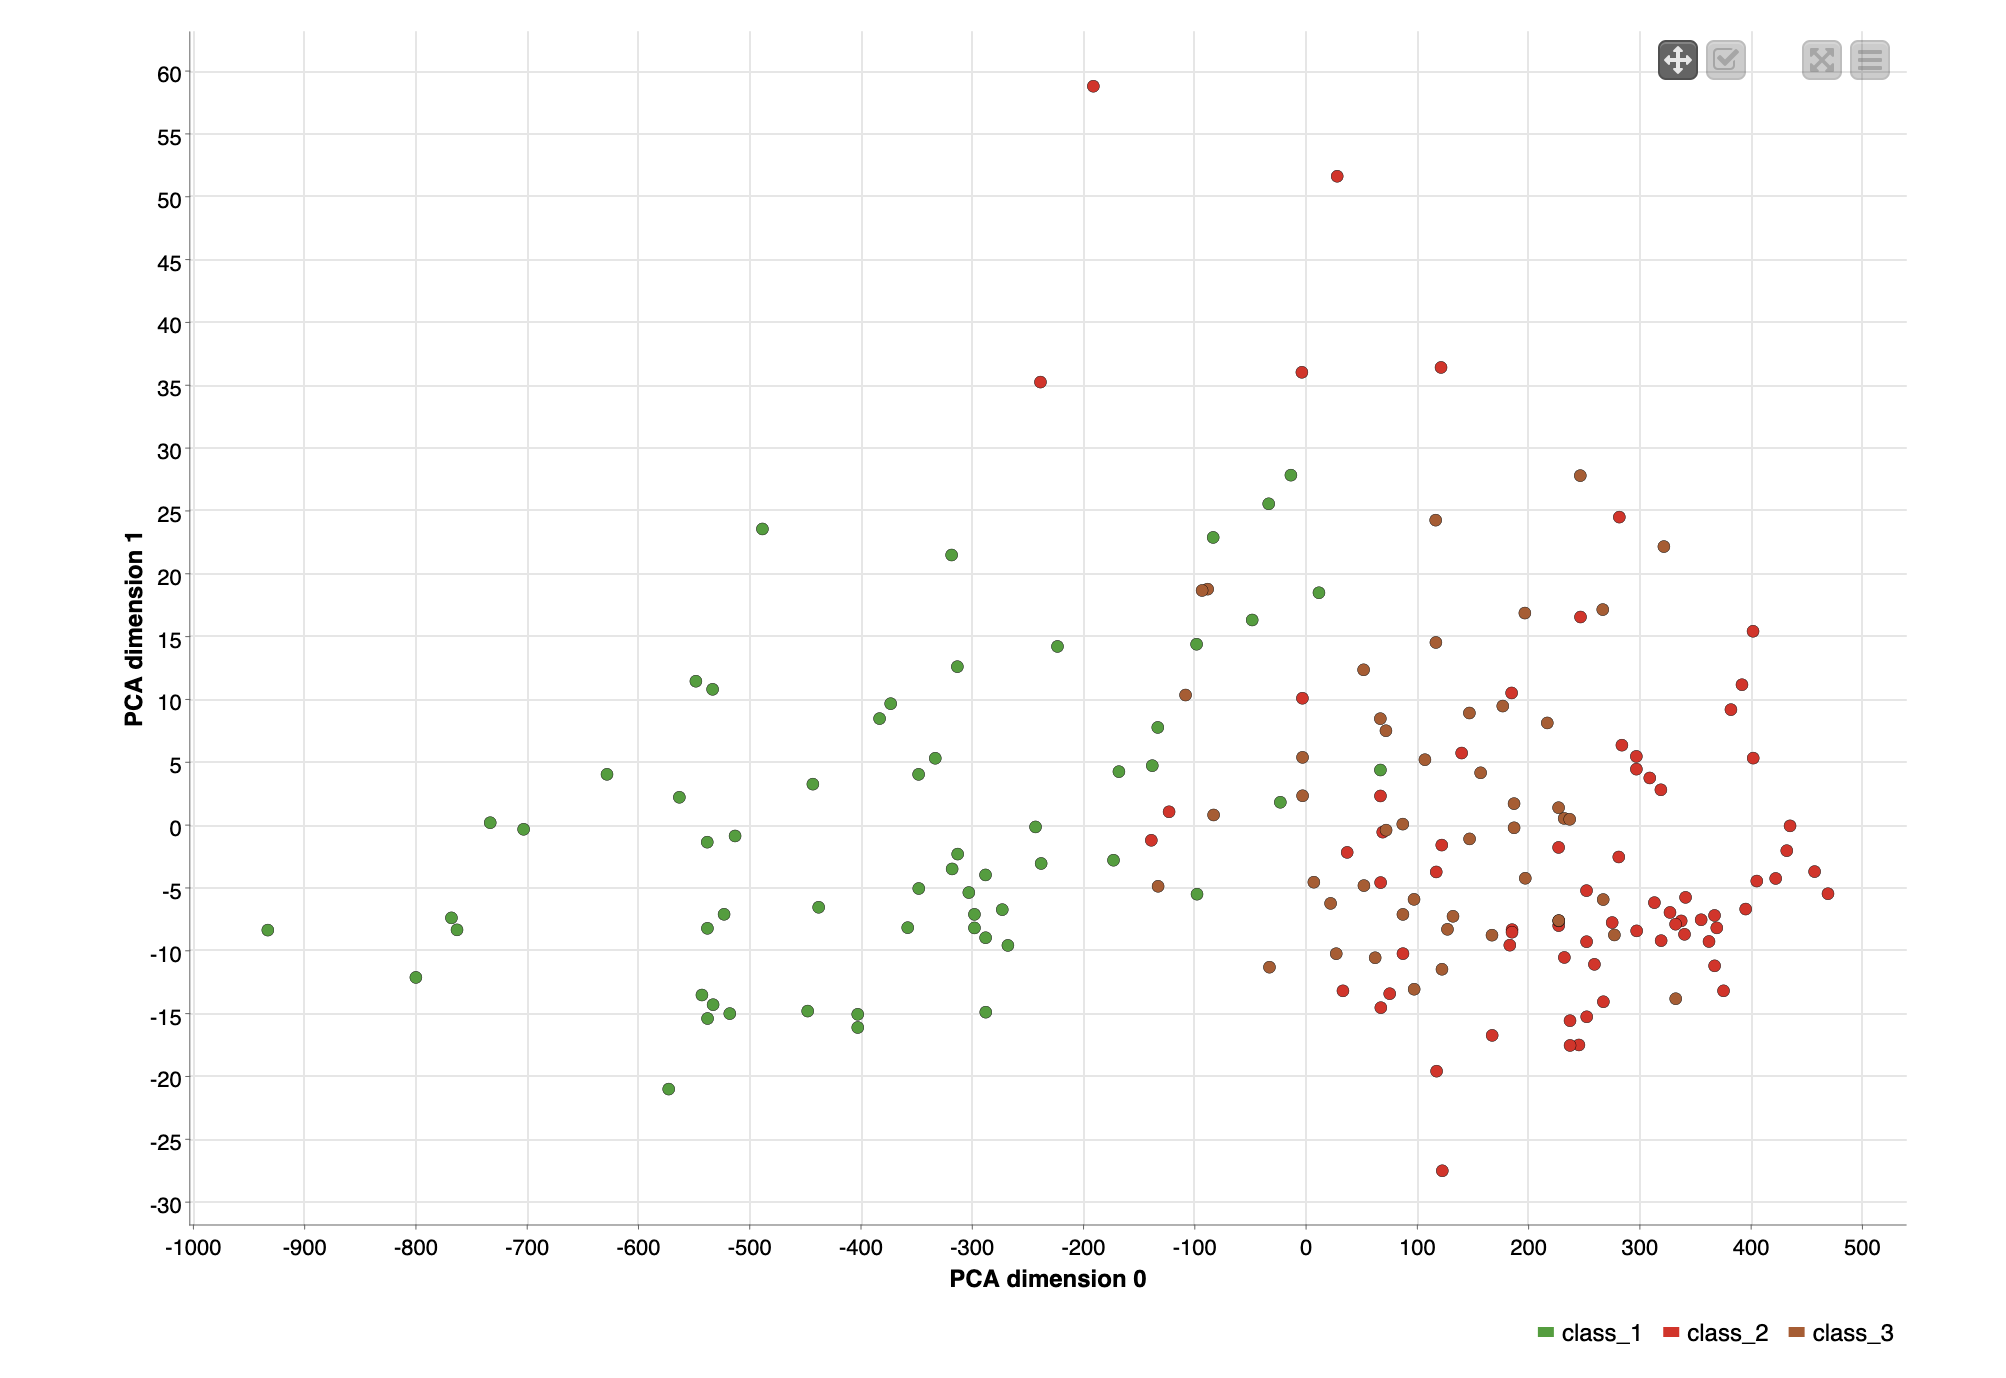
\includegraphics[scale=0.36]{res/plot1.1}
	 
	 \section*{Task 1.2 : plot2}
	 
	% 	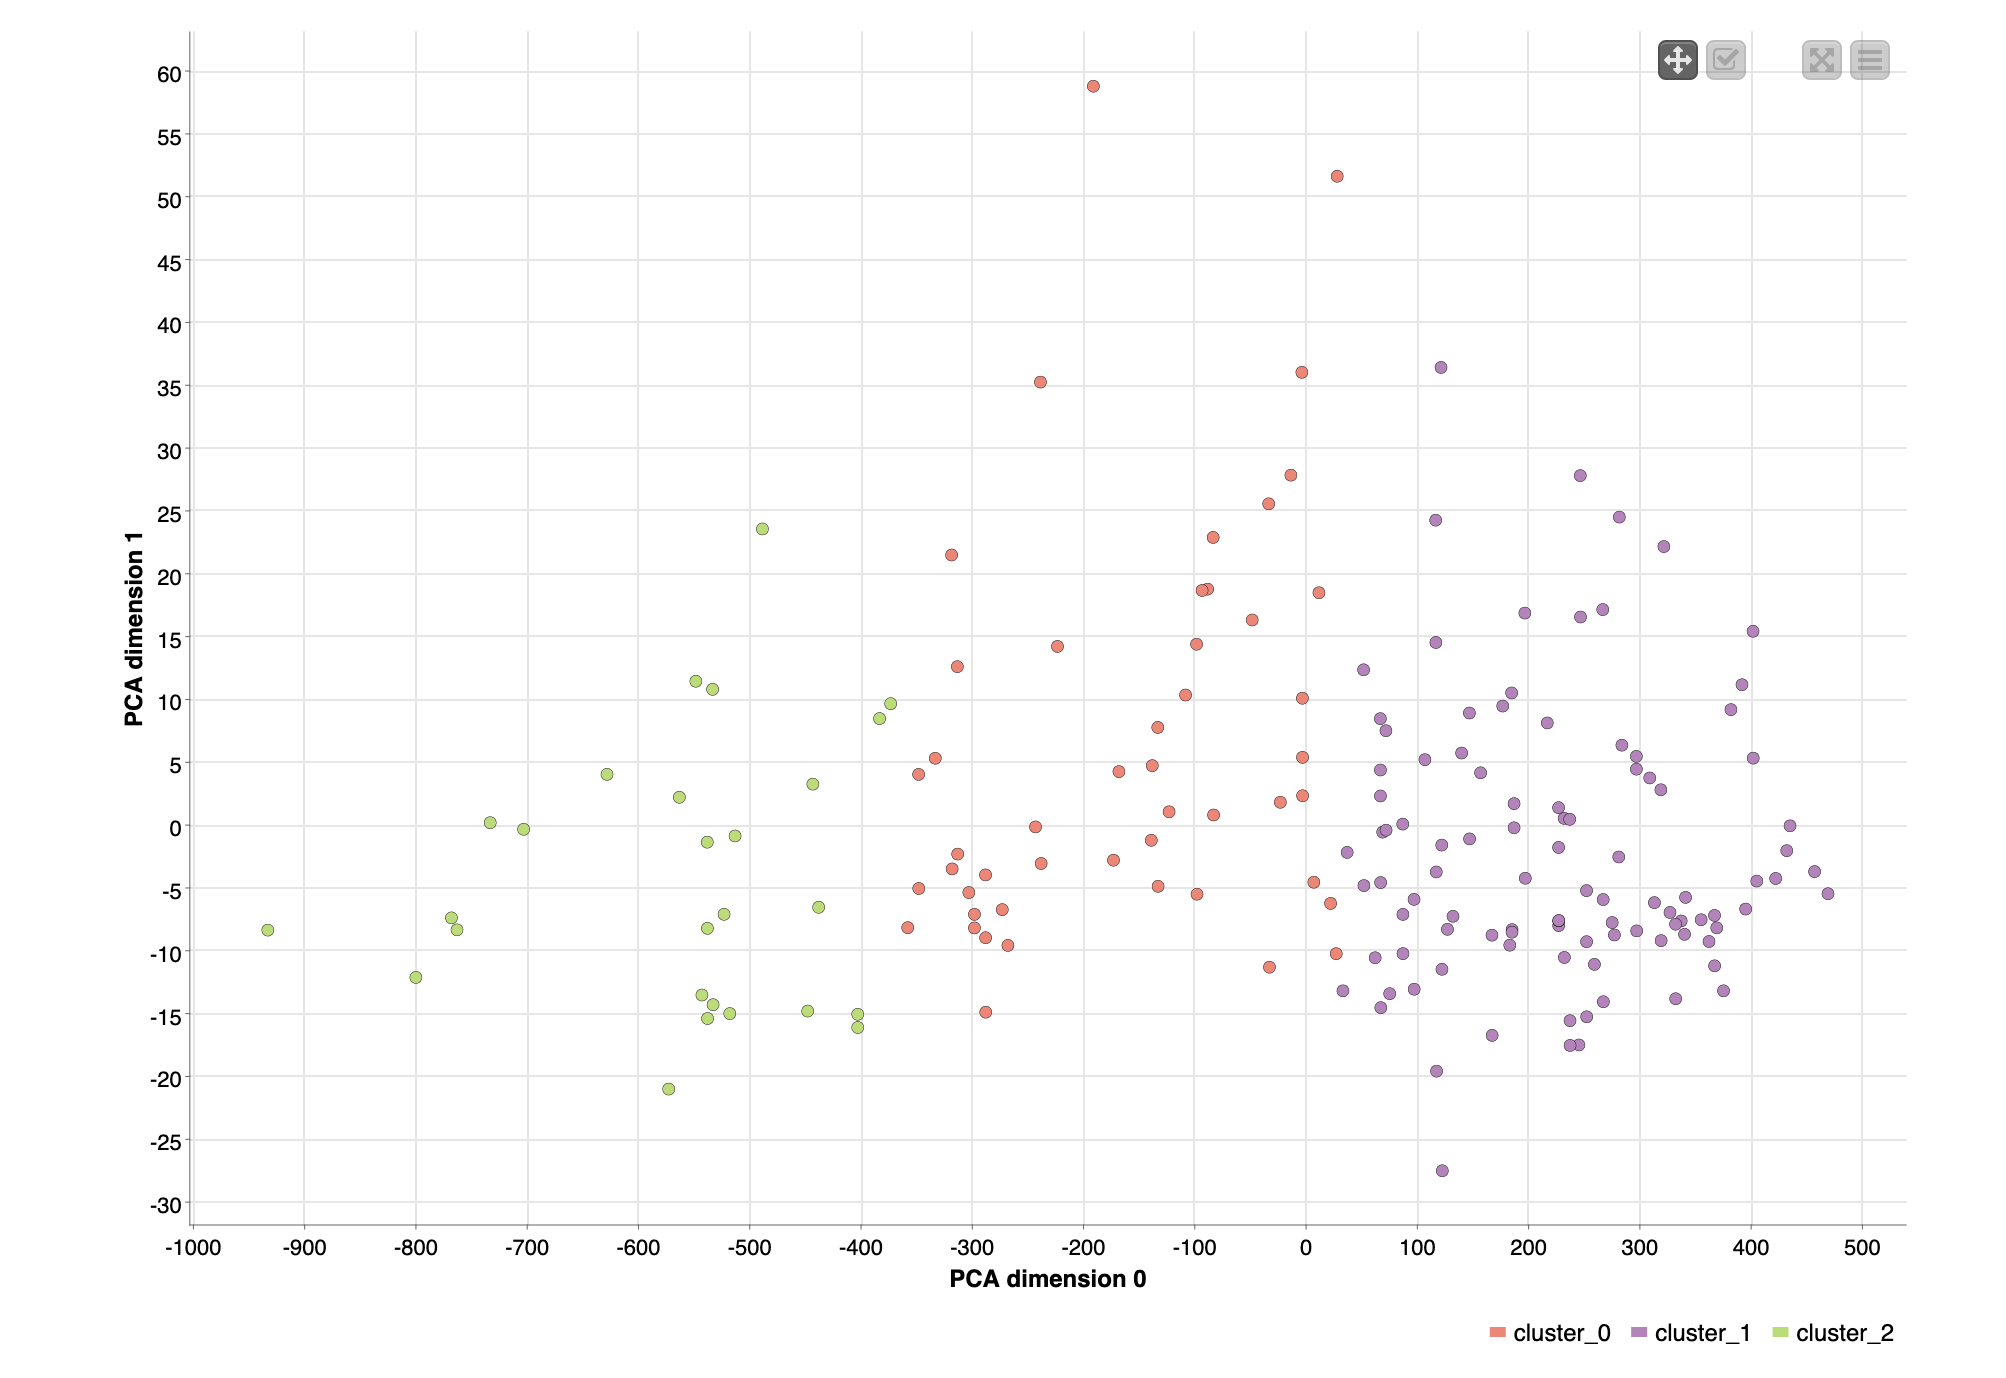
\includegraphics[scale=0.36]{res/plot1.2}
	 
	 \section*{Task 1.3 : compare, discuss and explain the differences between plot1 and plot2}
		The main point of interest in the figures above, is the fact that, the clustering algorithm(K-Means, k=3) failed to appropriately partition the data, and recognise the classes provided by the dataset. We can see that there are multiple errors(Detailed analysis per-class on Task 1.4). This phenomenon can be explained due to the absence of the standardization process, something that will be explained in the next Task. The exact scale of the problem cannot be appropriately assessed with only those two plots though, we will need to examine the distribution of the classes in each cluster, something that will be done on the next task(Task 1.4)
	
	 \section*{Task 1.4 : plot3a,plot3b,plot3c}
		The 3 requested plots are shown below
		 \begin{figure}[H]
		 	\centering
		 	\begin{subfigure}{0.4\textwidth}
	%	 		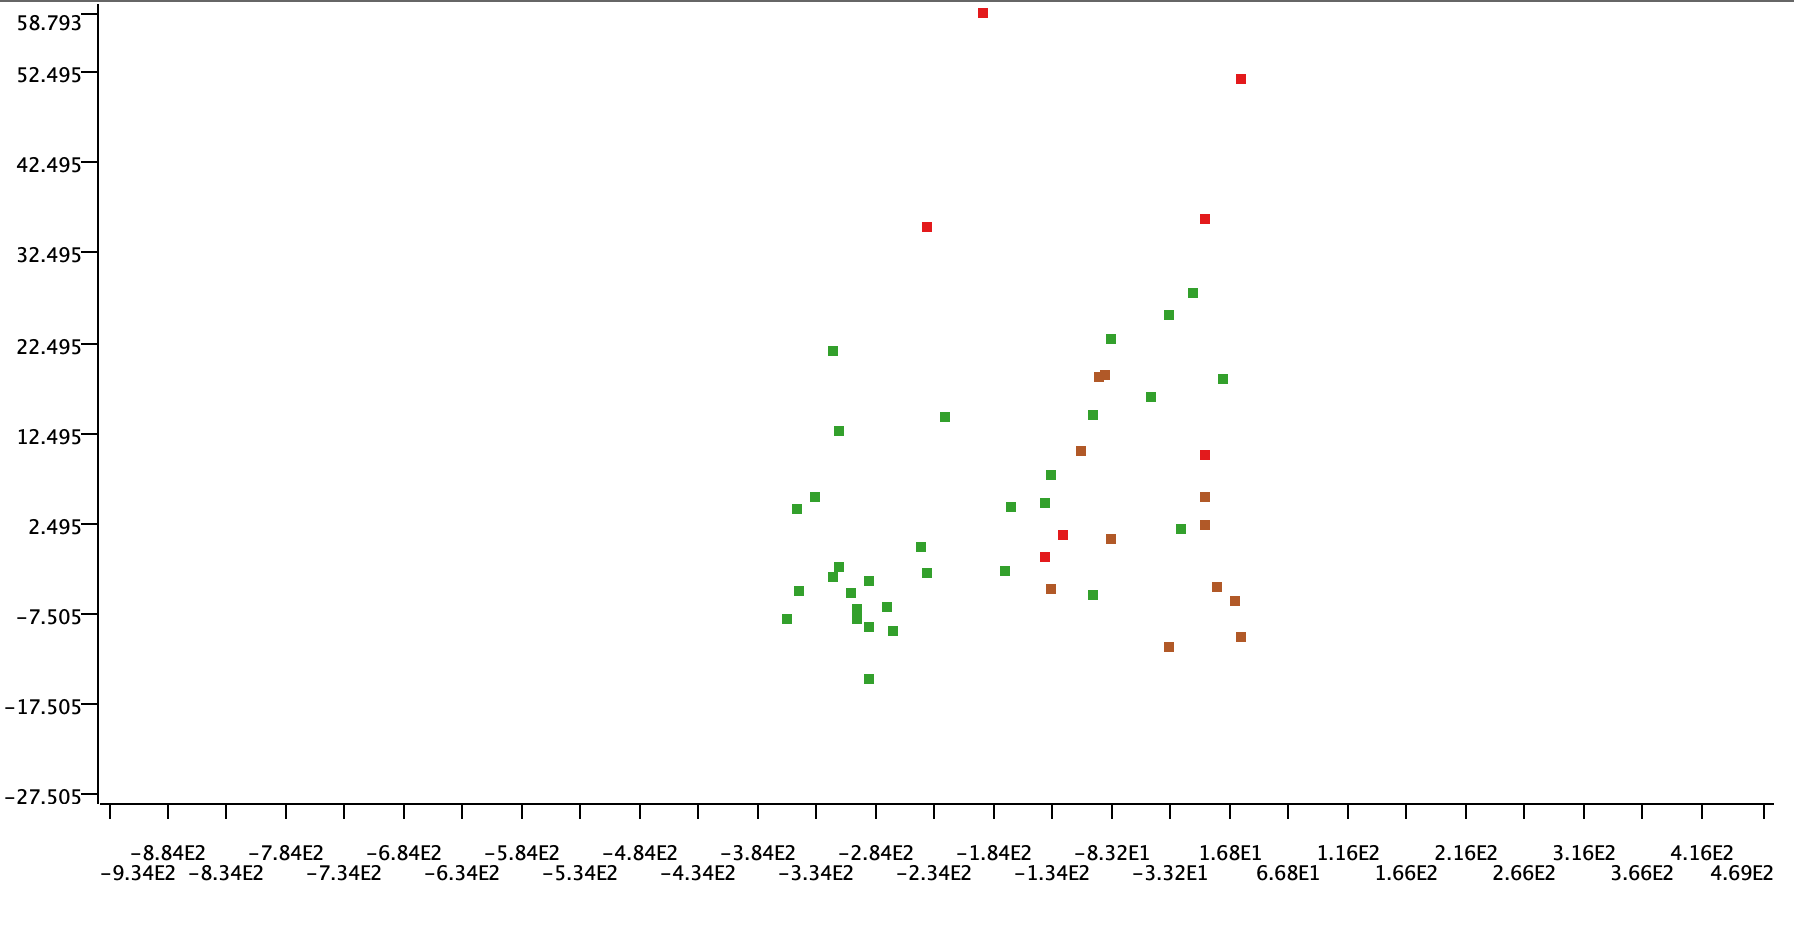
\includegraphics[width=\textwidth]{res/plot3a}
		 		\caption{plot3a}
		 		\label{fig:first}
		 	\end{subfigure}
		 	\hfill
		 	\begin{subfigure}{0.4\textwidth}
%		 		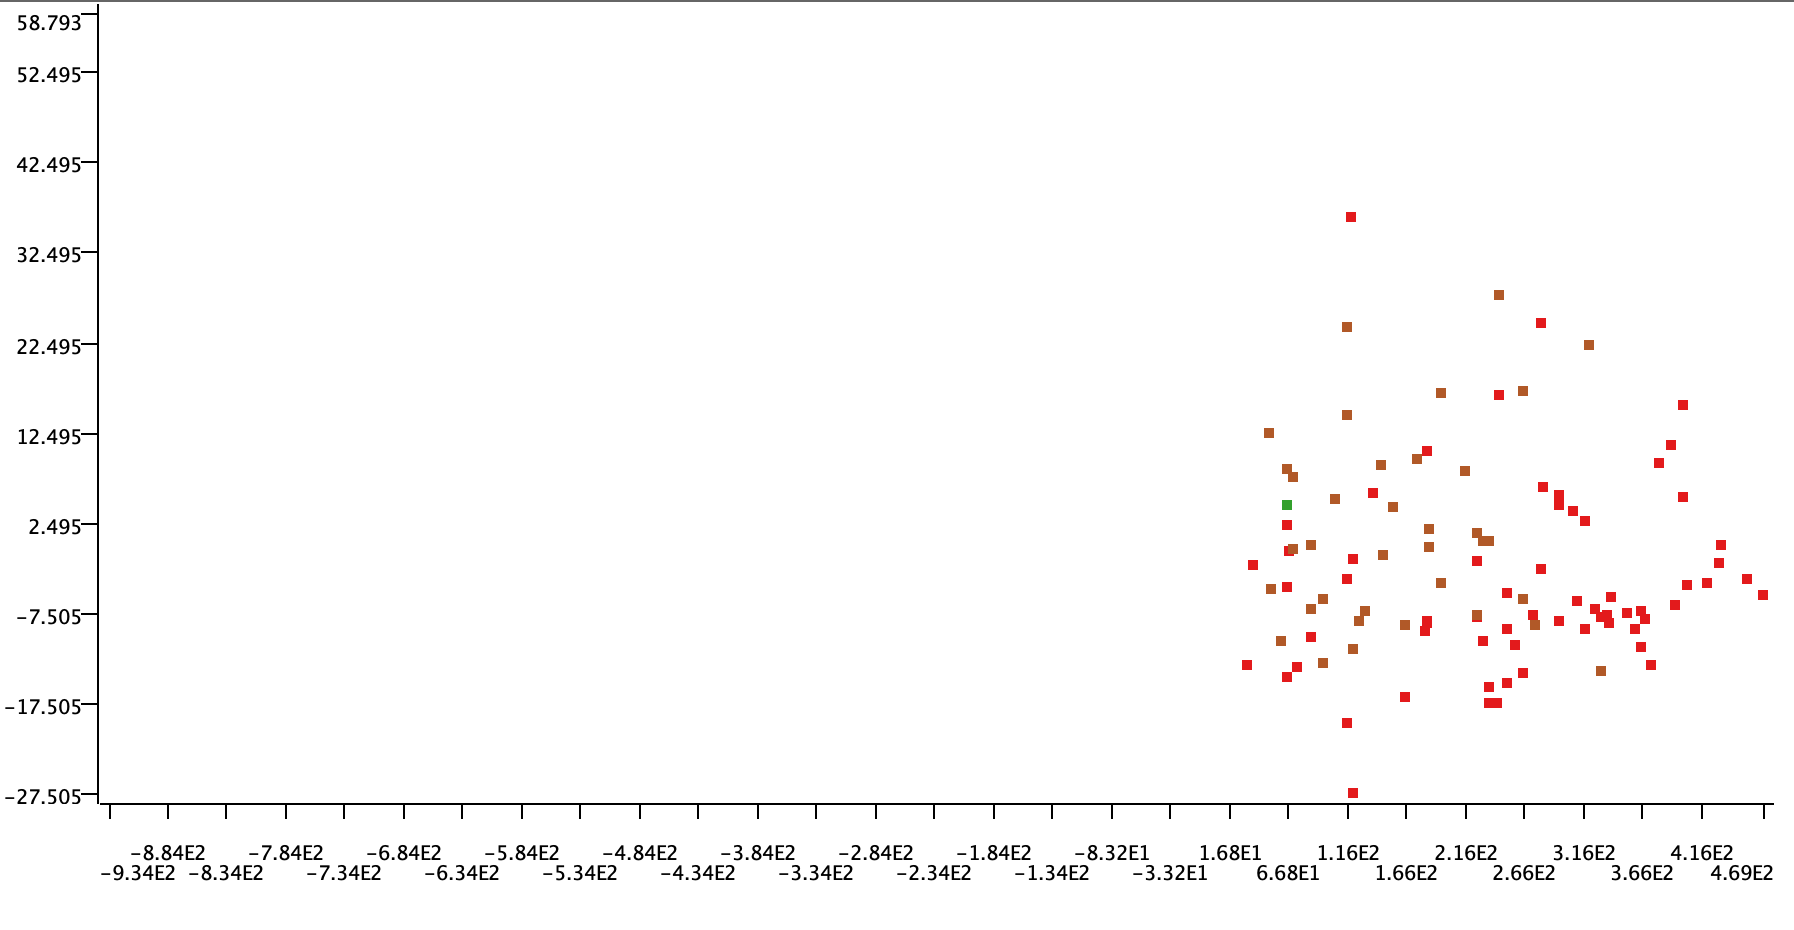
\includegraphics[width=\textwidth]{res/plot3b}
		 		\caption{plot3b}
		 		\label{fig:second}
		 	\end{subfigure}
		 	\hfill
		 	\begin{subfigure}{0.4\textwidth}
%		 		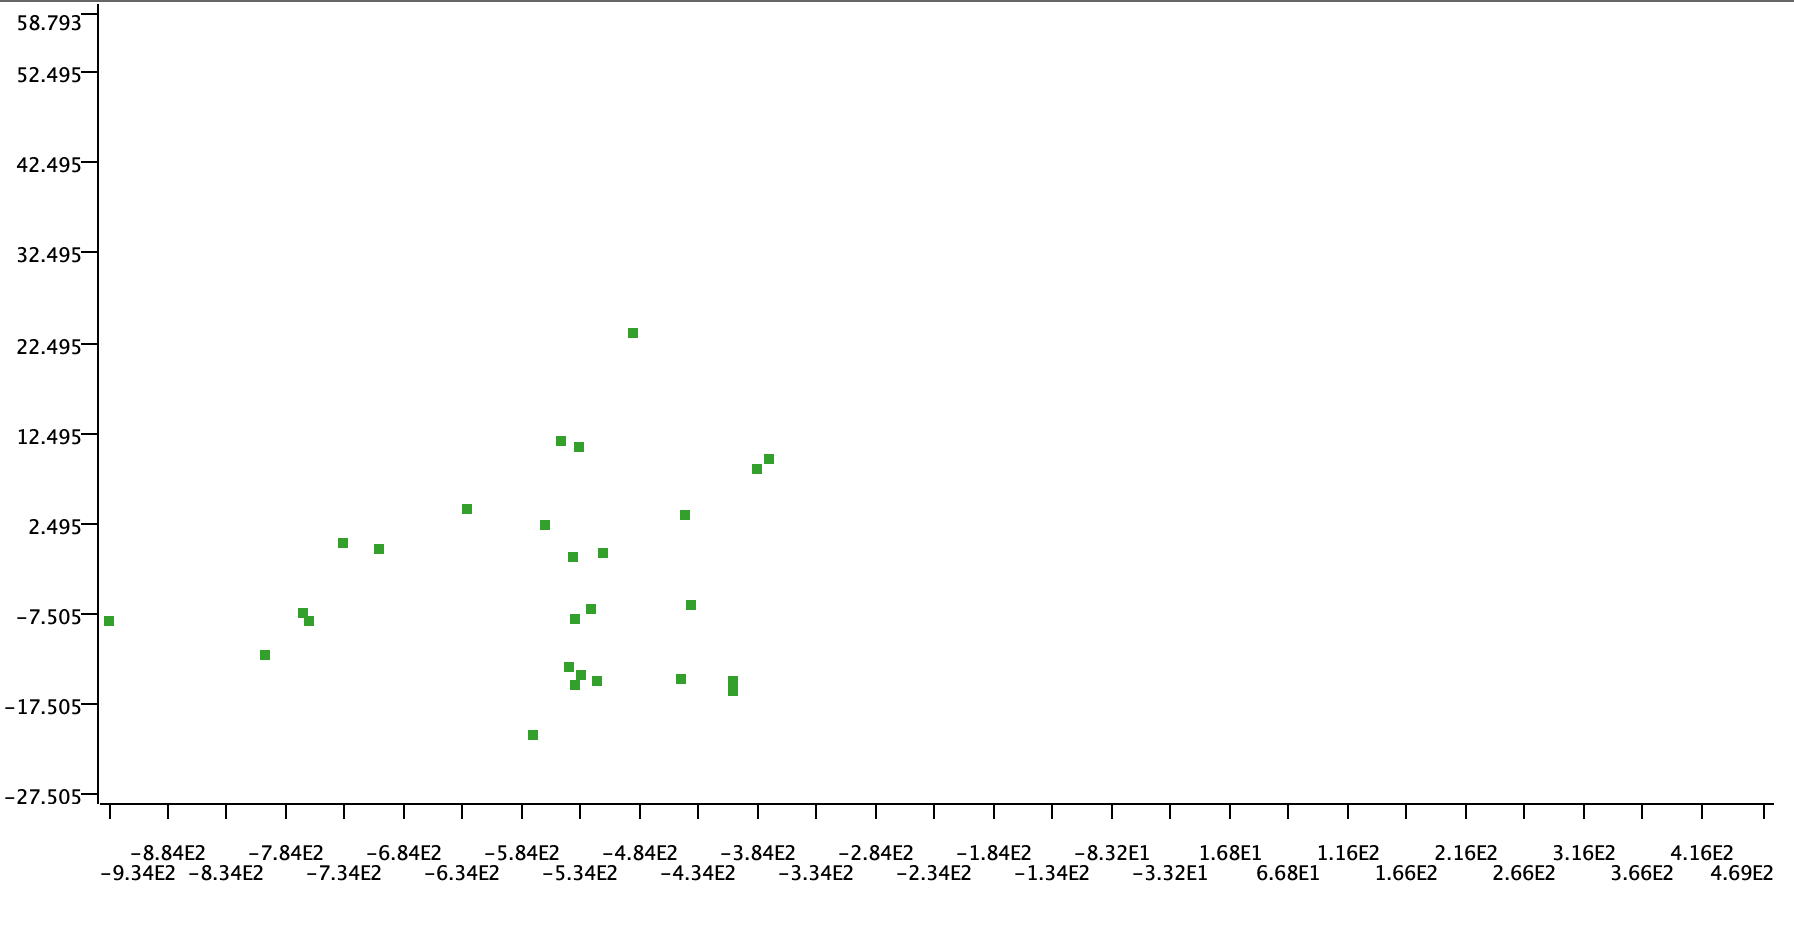
\includegraphics[width=\textwidth]{res/plot3c}
		 		\caption{plot3c}
		 		\label{fig:third}
		 	\end{subfigure}
		 	
		 	\label{fig:figures}
		 \end{figure}
		Here, we can see clearly each cluster and the classes of each datapoint that fails under those clusters. With use of histograms, we can learn the distribution of of classes in each cluster. Under ideal conditions(a good clustering), each cluster will contain the majority of the datapoints for some class, with a few missed points, unfortunately, this is not the case
		\begin{figure}[H]
			\centering
			\begin{subfigure}{0.4\textwidth}
%				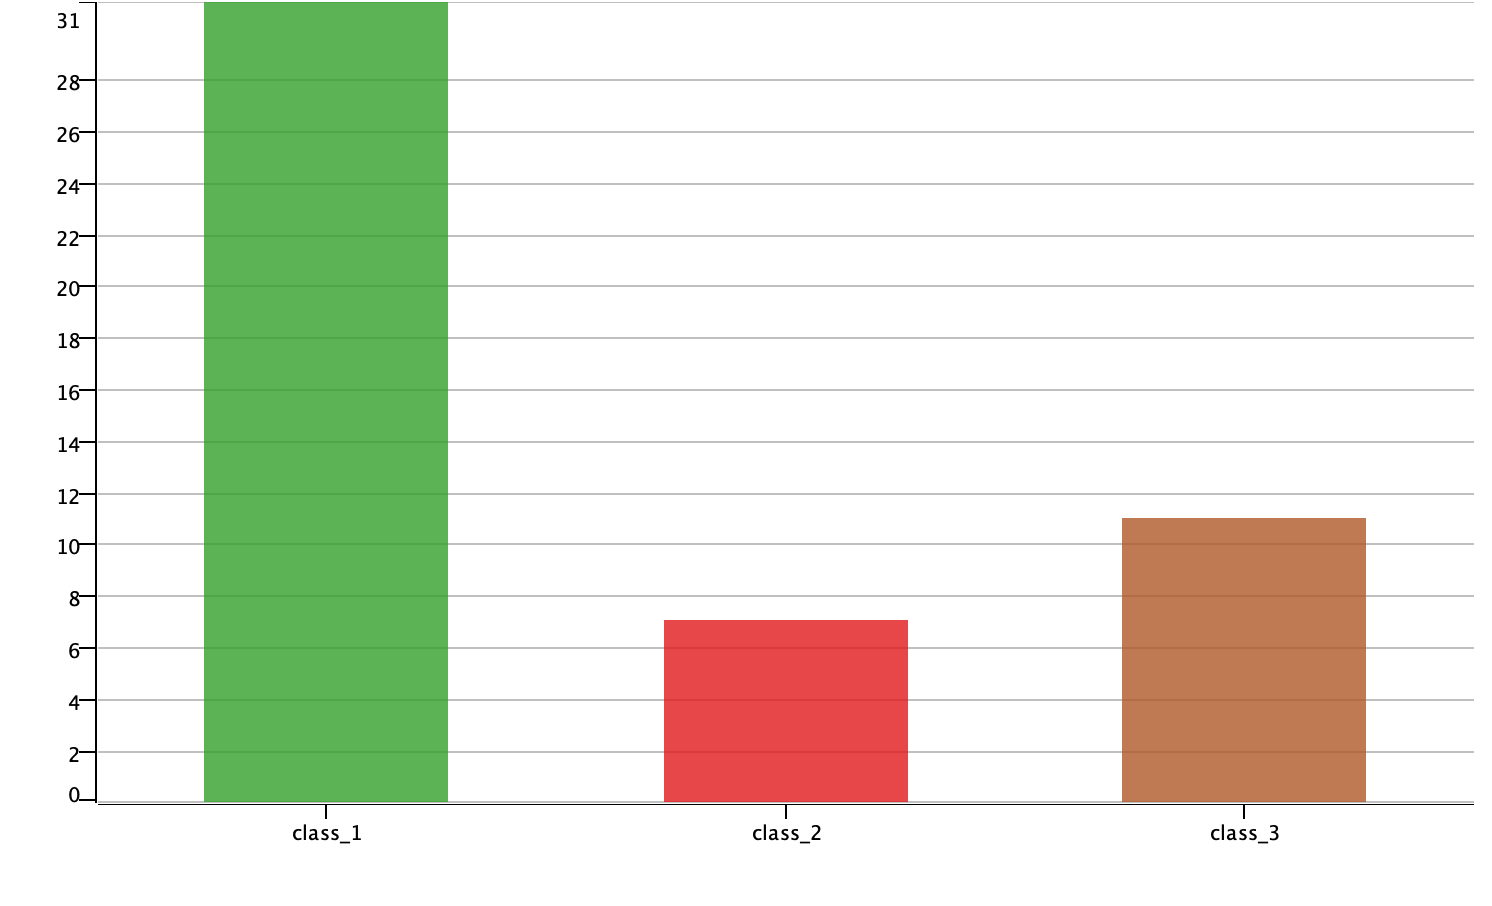
\includegraphics[width=\textwidth]{res/plot3adist}
				\caption{plot3a distribution}
				\label{fig:first}
			\end{subfigure}
			\hfill
			\begin{subfigure}{0.4\textwidth}
%				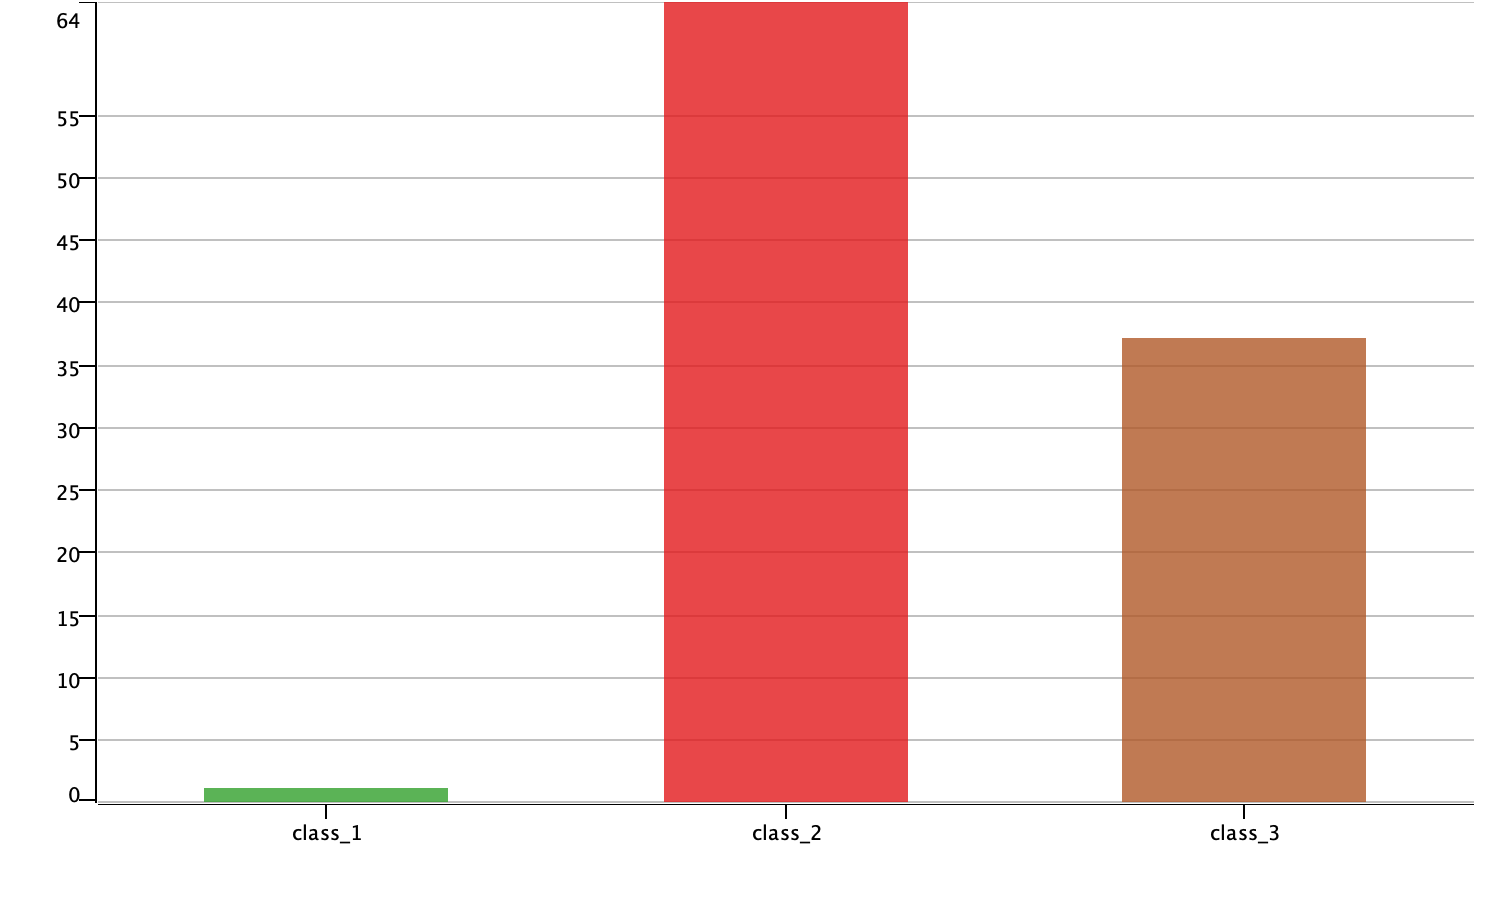
\includegraphics[width=\textwidth]{res/plot3bdist}
				\caption{plot3b distribution}
				\label{fig:second}
			\end{subfigure}
			\hfill
			\begin{subfigure}{0.4\textwidth}
%				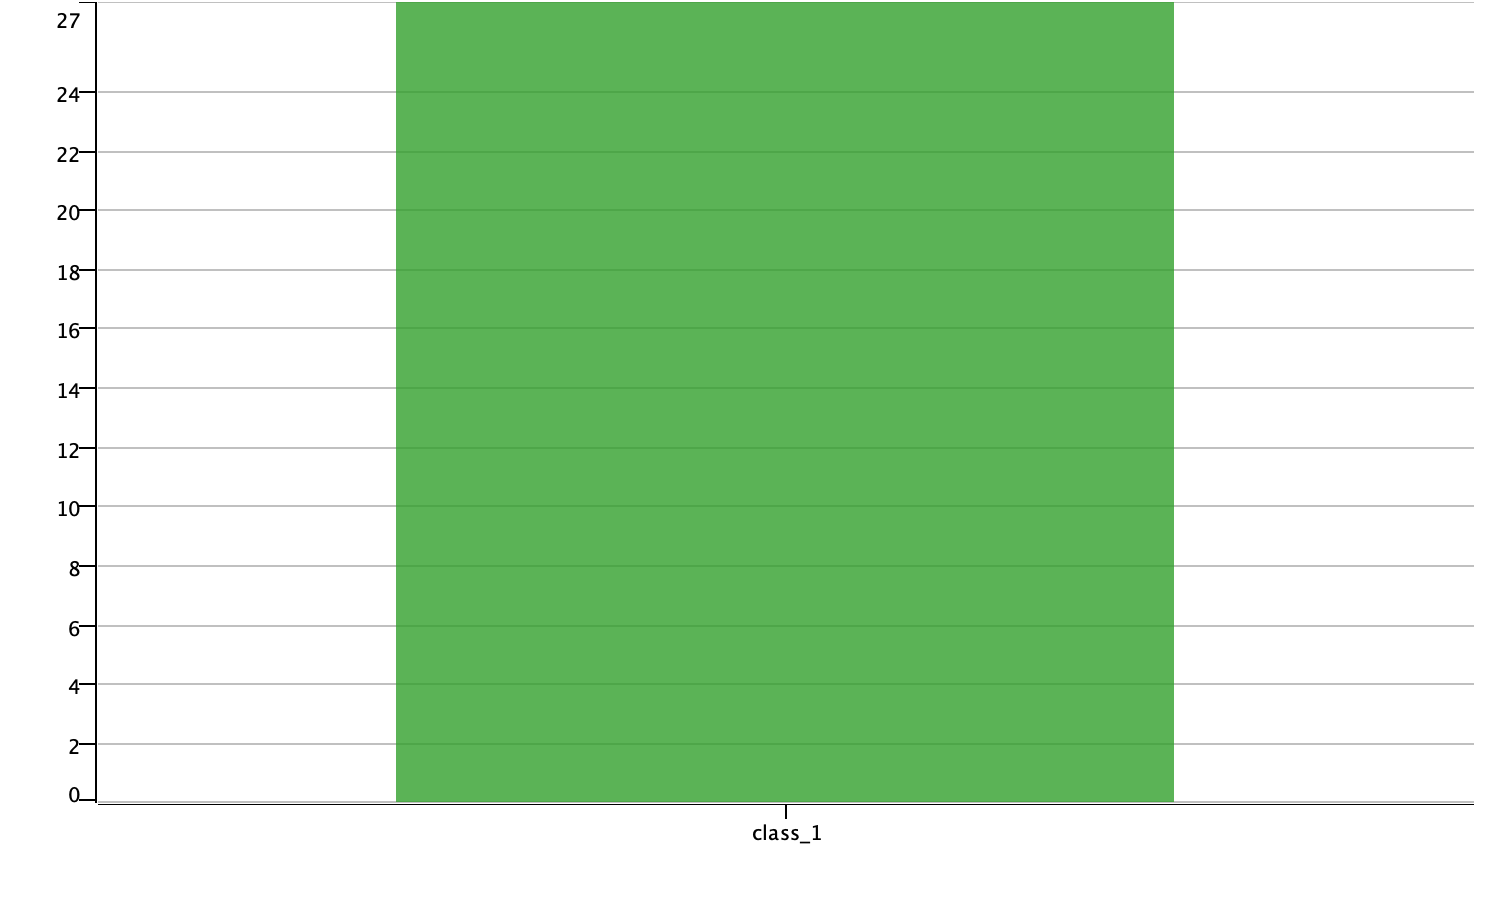
\includegraphics[width=\textwidth]{res/plot3cdist}
				\caption{plot3c distribution}
				\label{fig:third}
			\end{subfigure}
			
			\label{fig:figures}
		\end{figure}
		 This is the result of the lack of a normalization/standarization process, something that we will explain on the next task.
		 
		 \section*{Task 1.5 : Cluster Validity Measure}
		 	For our cluster validity measure, we will explain and intepret WSS (Within cluster sum of squares) and BSS (Between cluster sum of squares)
			\subsection*{Prerequisite 1 : Sum of Square Estimate of Errors(SSE)}
				Before our attempt of explaining WSS and BSS, it is essential to explain SSE (Sum of Square estimate of Errors). SSE is an evaluation metric with a plethora of applications in statistics and predictive analytics. It is used to evaluate a model's performance against a training set. The logic behind
				SSE is rather simple in nature. Let X an random variable and a model $y=\bar{X}$
				\begin{center}
%					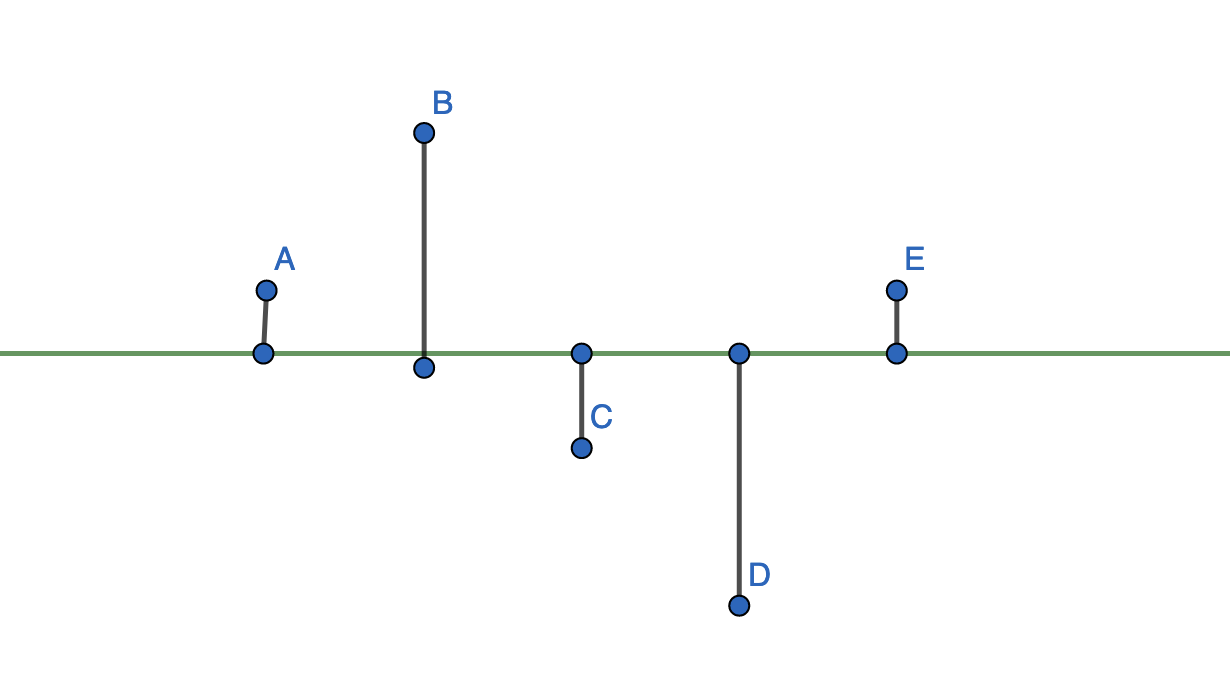
\includegraphics[scale=0.5]{res/SSE-1}
				\end{center}
				We can evaluate our model's performance, by calculating the Sum of Errors, where 'error' in this case, is the distance of the observed variable from the responce of our model (i.e the mean $\bar{X}$), as follows
				\begin{align}
					SE = \sum_{i=1}^{n}{X_i-\bar{X}}
				\end{align}
				Unfortunately, our evaluation metric has a fatal flaw, it allows for error's to 'cancel out' simply because they are placed beneath our model's line. It can be proven that, for the case of $y=\bar{X}$ SE is always 0.
				\begin{align}
					SE = \sum_{i=1}^{n}{X_i-\bar{X}} \\
					SE = \sum_{i=1}^{n}{X_i} - \sum_{i=1}{n}{\bar{X}} \\
					SE = \sum_{i=1}^{n}{X_i} - n\bar{X} \\
					SE = \sum_{i=1}^{n}{X_i} - \sum_{i=1}^{n}{X_i} \\
					SE = 0 \\
				\end{align}
				For other models(in higher dimensions, where corellation of the involved variables is not 1), it may not be zero, but the fatal flaw remains, by cancelling errors we severely underestimate the errors involved. A more appropriate approach could be to square the distances, that would give us the Sum of Squared Errors (SSE)
				\begin{align}
					SE = \sum_{i=1}^{n}{(X_i-\bar{X})}^2
				\end{align}
		 	\subsection*{WSS and BSS}
		 		In the world of Clustering models performance evaluation, SSE is translated into two distinct but related ideas, WSS and BSS
			%	\includegraphics[scale=0.5]{res/WSS-BSS-TSS}
		 		\subsubsection{WSS}
		 			WSS or  Within Cluster Sum of Squares is a clustering model performance evaluation function. Our 'model' in this case is the cluster centroid and the error 
		 		
		 		In context of Clustering, SSE WSS or Within Cluster Sum of Squares is , our 'model' is the estimated cluster center, and the 'errors' are calculated based on the distance of every datapoint of the cluster, to the estimated cluster center. A good clustering always aims for low WSS. The SSE variant of WSS is calculated as follows
		 		\begin{align}
sf=12					
		 		\end{align}
			\subsection*{BSS}
				whohoo
		
	
	
	%which leaves the algorithm vulnerable to distortion due to the different scales, measurement units and sizes of the variables in question. The following figure is part of the output of a simple 'Statistics' Node
	%Without Normalization
	%\begin{table}[H]
	%	\begin{tabular}{llllllllllll}
	%		Column&Min &Mean &	Median & Max  & Std. Dev.  \\
	%		Hue&0.48&0.9574&?&1.71&0.2286 \\
	%		Proline&278&746.8933&?&1,680&314.9075 \\
	%		&  &  &  & 
	%	\end{tabular}
	%\end{table}
	 
	
	
		
	
	\pagebreak
	\begin{thebibliography}{1}	
		\bibitem{entropy}
		\textit{Shannon, C., 1948. A Mathematical Theory of Communication. Bell System Technical Journal, 27(3), pp.379-423.}
		
	\end{thebibliography}
\end{document}
